\documentclass{article}
\usepackage[utf8]{inputenc}
\usepackage{polski}
\usepackage{graphicx} 

\title{AM1 - Zestaw 7}
\author{Wojciech Szlosek}
\date{April 2020}

\begin{document}
\section{FUNKCJA DO ZADANIA 1 (b)}
\begin{figure} 
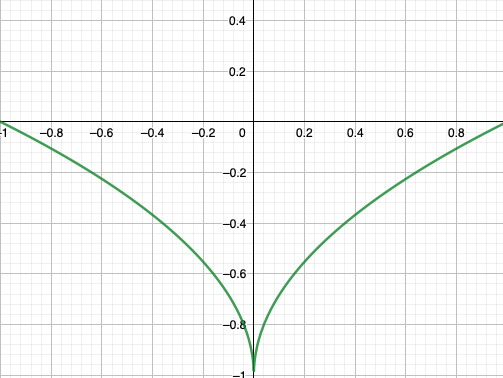
\includegraphics {funkcja.png} \end{figure} \newline \newline

\maketitle

\section{Zadanie 1 (b)}

$$g(x) = \sqrt{|x|} - 1 =\left\{ \begin{array}{rl}
\sqrt{-x}-1 & \textrm{dla $x<0$} \\ \sqrt{x}-1 & \textrm{dla $x\geq0$} \end{array}$$
\newline

Funkcja ta jest ciągła na przedziale $[-1,1]$. Jednak nie ma pochodnej w przedziale $(-1,1)$, ponieważ $g^{'}(0)$ nie istnieje: \newline

$$g^{'}_{+}(0) = \infty$$
$$g^{'}_{-}(0) = -\infty$$ \newline

Funkcja $g$ nie spełnia założeń twierdzenia Rolle`a na przedziale $[-1,1]$ \newline

\section{Zadanie 9 (a)}

$$x_0 = 2; n = 3$$
$$f(x) = \frac{1}{x}$$

$$f^{'}(x) = (x^{-1})^{'} = -x^{-2} = \frac{-1}{x^2}$$

$$f^{''}(x) = -(x^{-2})^{'} = \frac{2}{x^3} $$

$$f^{'''}(x) = 2(x^{-3})^{'} = \frac{-6}{x^4} $$ \newline
Stąd $f(2) = \frac{1}{2}$, $f^{'}(2) = \frac{-1}{4}$,
$f^{''}(2) = \frac{1}{4}$ \newline
Wzór Taylora dla funkcji f przyjmuje postać: \newline
$$\frac{1}{x} = \frac{1}{2} +\frac{\frac{-1}{4}}{1!}(x-2) + \frac{\frac{1}{4}}{2!}(x-2)^{2} + \frac{\frac{-6}{c^{4}}}{3!}(x-2)^{3} = \frac{1}{2} -\frac{1}{4}(x-2)+\frac{1}{8}(x-2)^{2} + R_{3}(x) $$ \newline

gdzie $R_{3}(x) = \frac{-(x-2)^3}{c^4}$, przy czym $c$ jest liczbą zawartą między 2 i x.

\section{Zadanie 10 (a)}

$f(x) = \cos{x}$, $f^{'}(x) = -\sin{x}$, $f^{''}(x) = -\cos{x}$, $f^{'''}(x) = \sin{x}$, $f^{''''}(x) = \cos{x}$, \newline $p$ - liczba całkowita.
\newline

$$f^{(k)}(x)=\left\{ \begin{array}{rl}
\cos{x} & \textrm{dla $k = 4p$} \\
-\sin{x} & \textrm{dla $k = 4p+1$}\\
-\cos{x} & \textrm{dla $k = 4p+2$}\\
\sin{x} & \textrm{dla $k = 4p+3$}\end{array}$$   Zatem: \newline

$$f^{(k)}(0)=\left\{ \begin{array}{rl}
1 & \textrm{dla $k = 4p$} \\
0 & \textrm{dla $k = 4p+1$}\\
-1 & \textrm{dla $k = 4p+2$}\\
0 & \textrm{dla $k = 4p+3$}\end{array}$$ \newline

Podstawmy do wzoru Maclaurina:

$$\cos{x} = 1 - \frac{x^2}{2!} + \frac{x^4}{4!} - \frac{x^6}{6!} + ... + R_{n}(x) $$ gdzie $R_{n}(x) = +/- \frac{x^n}{n!}\left\{ \begin{array}{rl}
\sin{c} \\
\cos{c} \end{array}\right\}$, przy czym $c$ jest zawarte między 0 i x. Warto dodać, że znak + lub - i funkcję $sin/cos$ dobieramy w zależności od $n$.

\end{document}